\documentclass[12pt]{article}
\usepackage{amsmath}
\usepackage{graphics}
\usepackage{figadds}

\textwidth 17cm
\textheight 24cm
\oddsidemargin 0cm
\topmargin -1cm
\def\z{{\bf z}}
\def\Z{{\bf Z}}
\def\y{{\bf y}}
\def\Y{{\bf Y}}
\def\x{{\bf x}}
\def\X{{\bf X}}
\def\w{{\bf w}}
\def\t{{\bf t}}
\def\T{{\bf T}}
\def\I{{\bf I}}
\def\S{{\bf S}}
\def\m{{\bf m}}
\def\A{\mathcal{A}}
\def\D{\mathcal{D}}
\def\squeeze{\itemsep=0pt\parskip=0pt}

\begin{document}
\section*{Backpropation learning: Exercise 5}
This exercise is based on C.M.Bishop: \emph{Pattern Recognition
and Machine Learning}, Chapter 5.

The objective of this exercise is to get a feel for the issues
related to initialization, step size and stopping criteria for
gradient descent learning of neural networks, and finally become
familiar with basic aspects of second order optimization.

Print and comment on the figures produced by the software {\sf
 main5a.m, main5b.m, main5c.m} as outlined below at the {\bf
 Checkpoints}.

\subsection*{Neural network model}


Let $\y(\x)$ be a function of the vector \x, where
$\x=(x_1,\ldots,x_d)^\top$. The functional form of $\y(\x)$ is
 a neural network (NN) with one hidden layer as shown in Figure \ref{NN.eps}. We have a data-set, $\D = \left\{ (\x^n,\t^n)
\right\}$, $ n=1,\ldots,N$ of $N$ corresponding values of inputs $\x^n$ and
targets $\t^n$. We wish to use the training data to learn the mapping $\t=\y(\x)+\mathbf{\epsilon}$, where $\mathbf{\epsilon}$ is the residual which we usual interpret as noise.

\begin{figure}[hb]
\center
\includegraphics[width=16cm]{NN.eps}
\caption{Neural network with one hidden layer.}
\label{NN.eps}
\end{figure}
The function is  given by
%
\begin{eqnarray} \label{eq:model}
  y_{k} &=& \sum_{j=0}^M w^{(2)}_{kj} z_j \;\; , \;\;z_0\equiv1\\
   z_j &=& g\left(\sum_{i=0}^d w^{(1)}_{ji} x_i \right) \;\; , \;\;x_0\equiv1 \ ,
\end{eqnarray}
%
where $y_k$ is the $k$'th output of the model, $z_j$ is the the $j$'th output of hidden units and $g(\cdot)$ is a nonlinear
sigmoid
function. The parameters that we a going to estimate are usually called weights. They are given as
$\w^{(1)}$ for the hidden layer and $\w^{(2)}$ for the output layer.
It should be noted that a bias is included in the output and hidden layer by having $z_0$ and $x_0$ set to
one.
In matrix notation this can also be expressed as
\begin{eqnarray}
  \label{eq:model}
  \y &=& (\w^{(2)})^\top \z \;\; , \;\;z_0\equiv1\\\
   \z &=& g\left((\w^{(1)})^\top \x \right) \;\; , \;\;x_0\equiv1 \ .
\end{eqnarray}
%
The optimal weights $\w$  are found by minimization of an error function.
Here we shall use the sum-of-squares error function augmented by a
weight-decay term
\begin{eqnarray}
  \label{eq:error1}
  E(\w) &=& \frac{1}{2} \sum_{n=1}^N \sum_{k=1}^{c}\left\{ y_k(\x^n;\w)-t_k^n \right\}^2 + \frac{1}{2}\alpha|\w|^2 \ .
\end{eqnarray}
The weight decay term, parametrized by $\alpha$, lowers the complexity of the model by shrinking the magnitude of the weights. Larger absolute weights makes the neural network mapping more non-linear and thus able to fit more different datasets including noise in the data. Adding the weight decay term can therefore help avoid overfitting.
%
\begin{figure}[ht]
\center
%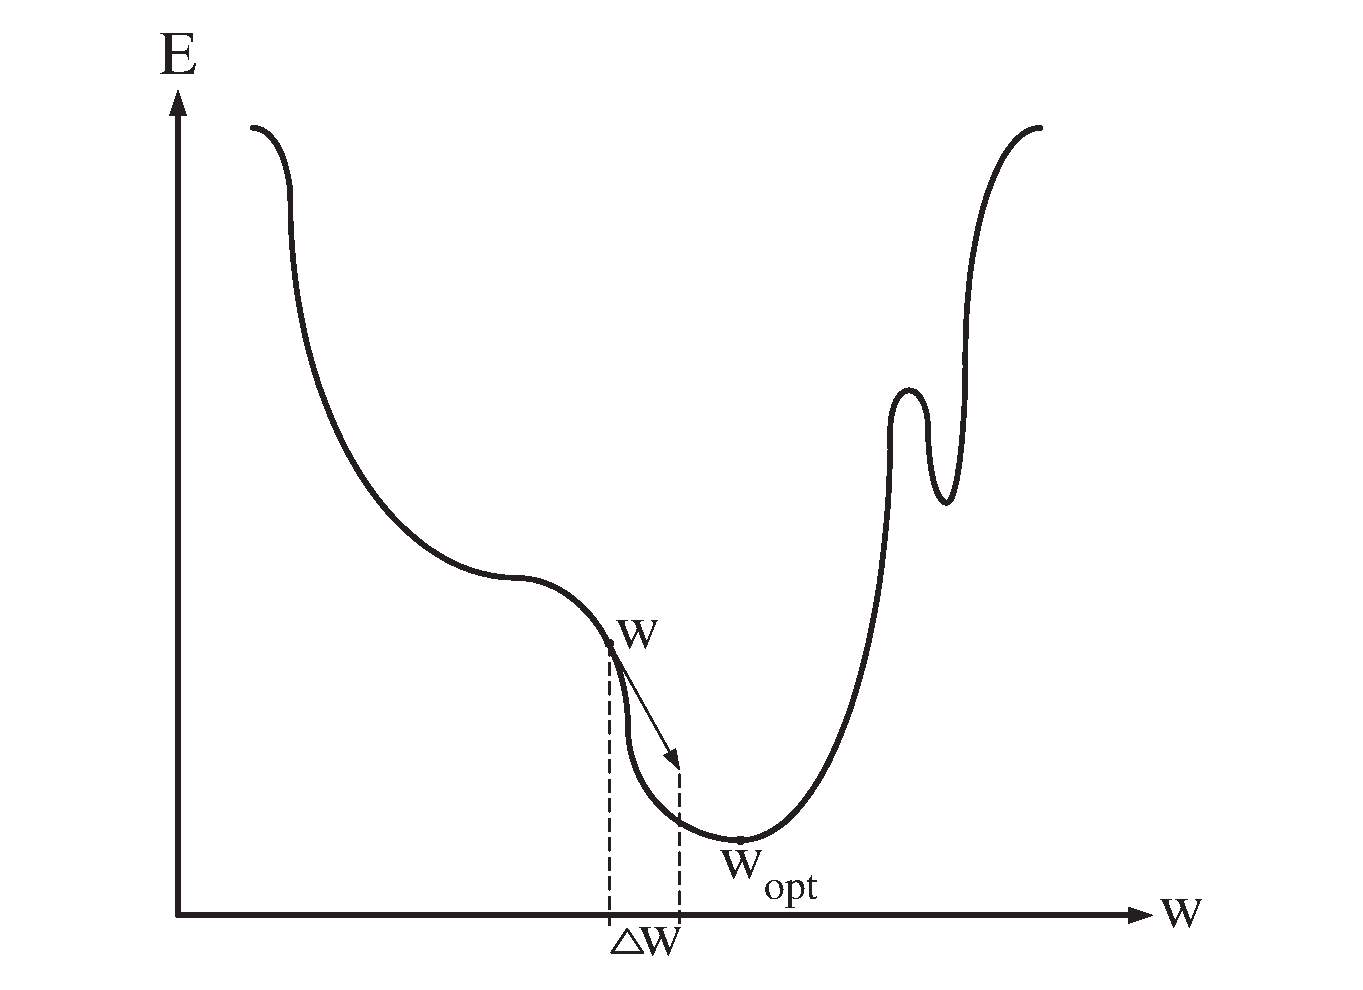
\includegraphics[width=8cm]{gradient.eps}
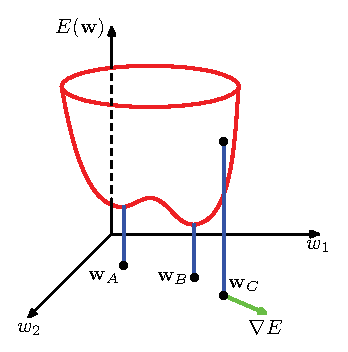
\includegraphics[width=8cm]{Bishop_figure5d5.eps}
\caption{The weight update is done by gradient descent going the
opposite direction of the cost functions gradient.}
\label{gradient.eps}
\end{figure}
%

Finding the optimal weights minimizing Eq.\ (\ref{eq:error1}) cannot be find analytically for the neural network model. An iterative scheme
\begin{eqnarray}
  \label{eq:gradient}
  \w_{new} &=&  \w_{old}+ \triangle \w 
\end{eqnarray}
is used instead. One choice for $\triangle \w$ is to move the weights in
 the opposite direction of the gradient of the error function Eq.\
(\ref{eq:error1}):
\begin{eqnarray}
  \label{eq:gradient}
  \triangle \w &=&  -\eta\frac{\partial E(\w)}{\partial \w} \ ,
\end{eqnarray}
where $\eta$ is the \emph{step size} parameter controlling
how long a step $\triangle \w$ should be. 
This method is called \emph{gradient descent} and is illustrated in Figure
\ref{gradient.eps}. Differentiating (\ref{eq:error1}) with
respect to the weights in the output and hidden layer gives
\begin{eqnarray}
  \label{eq:output}
  \triangle w_{kj}^{(2)} &=&  -\eta \left( \sum_{n=1}^N (y_{nk}-t_{nk}) z_{nj} + \alpha w^{(2)}_{kj} \right) \\
  \label{eq:hidden}
  \triangle w_{ji}^{(1)} &=&  -\eta \left( \sum_{n=1}^N\left((1-z^2_{nj})\sum_{k=1}^{c}w_{kj}^{(2)}(y_{nk}-t_{nk})\right)x_{ni} + \alpha w_{ji}^{(1)} \right)
\end{eqnarray}
%
\iffalse{
\begin{eqnarray}
  \label{eq:output}
  \triangle w_{kj} &=&  -\eta \sum_{n} (y_k-t_k) z_j + \alpha w_{kj}\\
  \label{eq:hidden}
  \triangle w_{ji} &=&  -\eta \sum_{n}\left((1-z^2_j)\sum_{k=1}^{c}w_{kj}(y_k-t_k)\right)x_i + \alpha w_{ji}
\end{eqnarray}
}\fi
%
using that the nonlinear function $g(a)=\tanh(a)$ shown in Figure
\ref{tanh.eps}.

In the following sections we want to investigate some of the
parameters involved in the optimization.

\begin{figure}[ht]
\center
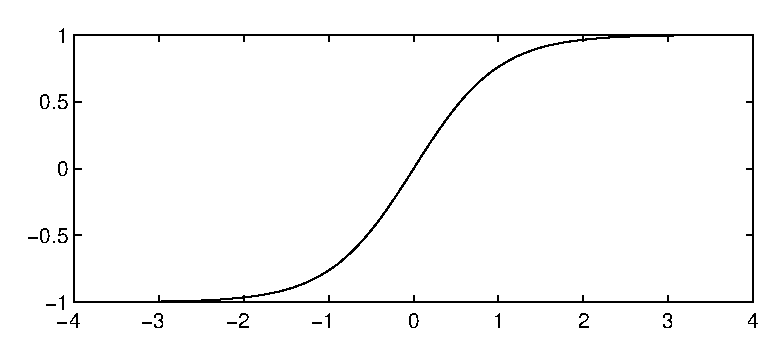
\includegraphics[width=8cm]{tanh.eps}
\caption{The nonlinear function $g(\cdot) = \tanh(\cdot)$.} \label{tanh.eps}
\end{figure}

\subsection*{Initialization range}
The gradient descent process starts from  an initial set of values for the weights.
 The role of the
initialization range is important for the convergence of
the parameters. If the range is making the initial weights too
small compared to the signal, the gradient will be small and learning slow initially. On the other hand, setting the
range to high forces the nonlinear function close to the step
function and again the gradients become small and learning slow.


\subsubsection*{Checkpoint 5.1:}
Use the program {\sf main5a.m} to create an NN training-set with a
4-dimensional input variable, 5-dimensional hidden variable and a
1-dimensional output variable ($4\times 5\times 1$). Observe the
effects of setting the range of the initial weights to: 0, 0.5 and
10000. Use Eqs.\ (\ref{eq:output},\ref{eq:hidden}) and Figure \ref{tanh.eps} to explain the effects you see.


\subsection*{Step size parameter}
 The step
size parameter $\eta$ can be chosen in various ways. In this exercise we use a
 fixed value throughout the iteration scheme. This is not optimal, and we shall look
 at better schemes in the last Checkpoint in this exercise. When the step size is large the NN can `overshoot'.
 To avoid this one might choose a small step size
value, but this tends to make the NN converge more slowly.

\subsubsection*{Checkpoint 5.2:}
Use the program {\sf main5a.m} to create an NN training-set with a
4-dimensional input variable, 5-dimensional hidden variable and a
1-dimensional output variable ($4\times 5\times 1$). Set the step size to different
values and observe the behavior. What is a good step size
for the data-set?


\subsection*{Stopping criteria}
Various methods can be used to stop the iteration process. The stopping criterion
depends on the application. Here we will consider two possible candidates.

\subsubsection*{Checkpoint 5.3:}
 Use the program {\sf main5b.m} to plot the test and training errors,
 the length of the gradient vector, and the training error
 difference between iterations. Comment on the plots and how they could be used as a
 stopping-criteria.


\subsection*{Improved optimization procedures}

Non-linear optimization is a very active area of research and there exist many algorithms non of which are uniformly superior. The best choice depends upon the problem at hand. Although this topic is not a part of the curriculum, a bit of background knowledge about this topic is important to have in your toolbox.
A subset of important algorithms are shown in
Table~\ref{tab:optim}. 
%
\begin{table}[bh]
  \begin{center}
    \begin{tabular}{cclp{5cm}}
      \hline\hline
      1st & 2nd & Name \\ \hline
      $-$ & $-$ & Amoebe / simplex / Nelder-Mead \\
      + & $-$ & {\bf Gradient descent} \\
      + & $-$ & Gradient descent with momentum \\
      + & $-$ & Natural gradient  \\ \hline
      + & $-$ & Conjugate gradient algorithm & \\
      & & ---  {\bf Hestenes-Stiefel} \\
      & & ---  {\bf Fletcher-Reeves} \\
      & & ---  {\bf Polak-Ribiere} \\
      & & ---  Scaled conjugate gradient &  \\ \hline
      + & $-$ & Quasi-Newton  \\
      & & --- Davidson-Fletcher-Powell (DFP)  \\
      & & --- Rank-one-formula  \\
      & & --- Broyden-Fletcher-Goldfarb-Shanno (BFGS)  \\
      \hline
      + & (+) & {\bf Pseudo(-Gauss)-Newton} \\
      + & (+) & Gauss-Newton \\
      + & + & Levenberg-Marquardt \\
      + & + & Newton(-Ralphson)  \\
      \hline \hline
    \end{tabular}
    \caption{Some optimization algorithms.}
    \label{tab:optim}
  \end{center}
\end{table}
%
Most of the algorithms in Table~\ref{tab:optim} use an iterative
scheme where the parameters ${\bf w}$ are initialized to some
values and then a step is taken to a new place
\begin{equation}
  \label{eq:step}
  {\bf w}^{(\tau+1)} = {\bf w}^{(\tau)} + \Delta {\bf w}^{(\tau)} \ .
\end{equation}
The usual {\em gradient descent} (used int eh previous Checkpoints) is the
negative gradient multiplied by a suitable learning rate $\eta$:
\begin{equation}
  \label{eq:backprob}
  \Delta {\bf w} = - \eta\ \frac{\partial E({\bf w})}{\partial {\bf w}} \ .
\end{equation}
One can develop the second order algorithms (Newton,
Levenberg-Marquardt, Gauss-Newton, pseudo-Gauss-Newton) from a
Taylor expansion up to the second order term of the cost function $E$
around $\hat{\bf w}$ :
\begin{equation}
  \label{eq:taylor}
  E({\bf w}) = E(\hat{\bf w}) + ({\bf w} - \hat{\bf w})' {\bf
    g}_{\hat{\bf w}} +
  \frac{1}{2} ({\bf w} - \hat{\bf w})' {\bf H}_{\hat{\bf w}} ({\bf w}
    - \hat{\bf w})
    + \ldots \ .
\end{equation}
${\bf g}_{\hat{\bf w}}$ is the first order derivative (gradient)
of the cost function in $\hat{\bf w}$ and ${\bf H}_{\hat{\bf w}}$
is the second order derivative---the Hessian---of the
cost function in $\hat{\bf w}$. The first order derivative with respect to
${\bf w}$ is:
\begin{equation}
  \label{eq:derivative}
  \nabla E({\bf w}) = {\bf g}_{\hat{\bf w}} + {\bf H}_{\hat{\bf
  w}} ({\bf w} - \hat{\bf w}) \ .
\end{equation}
We want to find a local minimum ${\bf w} = {\bf w}_0$. The
gradient should be zero there: $\nabla E ({\bf w}_0) = 0$, which
means that we can now isolate ${\bf w}_0$:
\begin{equation}
  \label{eq:zero}
  {\bf w}_0 = \hat{\bf w} + (- {\bf H}^{-1}_{\hat{\bf w}} {\bf
  g}_{\hat{\bf w}}) \ .
\end{equation}
Taking this step is the (full) Newton algorithm. The other second
order methods (and the quasi-Newton methods) use some kind of
approximation to the Hessian, e.g., the {\em pseudo-Gauss-Newton}
uses only the diagonal of the Hessian (here for each variable
$w_i$ in ${\bf w}$):
\begin{equation}
  \label{eq:pseudogn}
  \Delta w_i = - \frac{\partial E}{\partial w_i} \left/
  \frac{\partial^2 E}{\partial w_i^2} \right. \ .
\end{equation}
%
{\em Conjugate gradient algorithms} construct a series of {\em
conjugate} directions ${\bf d}$. These are direction that satisfy
the following condition:
\begin{equation}
  \label{eq:conj}
  {\bf d}'_{j+1} {\bf H} {\bf d}_j = 0 \ .
\end{equation}
There are three classic conjugate gradient algorithms,
Hestenes-Stiefel, Fletcher-Reeves and Polak-Ribiere, which
construct the series of conjugate directions using the following
equations (${\bf g}$ is the gradient):
\begin{eqnarray}
  \label{eq:conjgrad}
  {\bf d}_{j+1} &=& - {\bf g}_{j+1} +
  \frac{{\bf g}_{j+1}' ({\bf g}_{j+1} - {\bf g}_j ) }{{{\bf d}_j}'
  ({\bf g}_{j+1} - {\bf g}_j)}{\bf d}_j \\
  {\bf d}_{j+1} &=& - {\bf g}_{j+1} +
  \frac{{\bf g}_{j+1}' {\bf g}_{j+1} }{
  {\bf g}_{j}'{\bf g}_j } {\bf d}_j \\
  {\bf d}_{j+1} &=& - {\bf g}_{j+1} +
  \frac{{\bf g}_{j+1}' ({\bf g}_{j+1} - {\bf g}_j ) }{{{\bf g}_j}'
  {\bf g}_j}{\bf d}_j \ .
\end{eqnarray}
%
The conjugate gradient algorithms usually require that the
cost function is minimized along the conjugate direction, thus a {\em line
search} is performed.

\subsection*{Optimization in the neural regression toolbox}

The neural regression toolbox implements five different
optimization algorithms presently: Gradient descent,
pseudo-Gauss-Newton and three conjugate gradient algorithms:
Hestenes-Stiefel (HS), Fletcher-Reeves (FR) and Polak-Ribiere
(PR). The function {\tt nr\_trainx} implements them all and {\tt
nr\_train} only implements the two first. The gradient descent
algorithm chooses the (negative) gradient as its direction and the
step size (Bishop: learning rate $\eta$) is determined by line
search using a sort of bisection: The gradient decent starts with
a step that is as long as the gradient (i.e., $\eta=1$) and then halves
it until the cost function is decreasing. The
pseudo-Gauss-Newton starts with a length determined by
equation~\ref{eq:pseudogn}. The line search for both of these
algorithms is implemented in {\tt
  nr\_linesear}.
The pseudo-Gauss-Newton presently starts with 10 gradient descent
steps so that it (hopefully!) will get into a region where the
second order derivative is well-behaved.

The conjugate gradient algorithms use another type of line search
algorithm: quadratic (parabolic) and cubic interpolation and
extrapolation. The line search is inexact and
the stopping criterion for it is the so-called Wolfe-Powell condition.

This kind of line search is implemented with {\tt nr\_linesearch}
(not the same as {\tt nr\_linesear}!).

The neural network is run on the sunspot data. There are 12 inputs
plus a bias unit, 3 hidden units and one output.


\subsubsection*{Checkpoint 5.4}

Use the program {\tt main5c.m} to investigate the speed of
convergence for the different algorithms. The program runs the
algorithms a couple of times (each with a different seed for the
initialization of the weights) and computes the average of the
cost function value. The evolution of the cost functions is
available in the variable {\tt E}.

Determine which is the best algorithm and comment on the shapes of the
curves.





\end{document}


\begin{figure}[ht]
\center
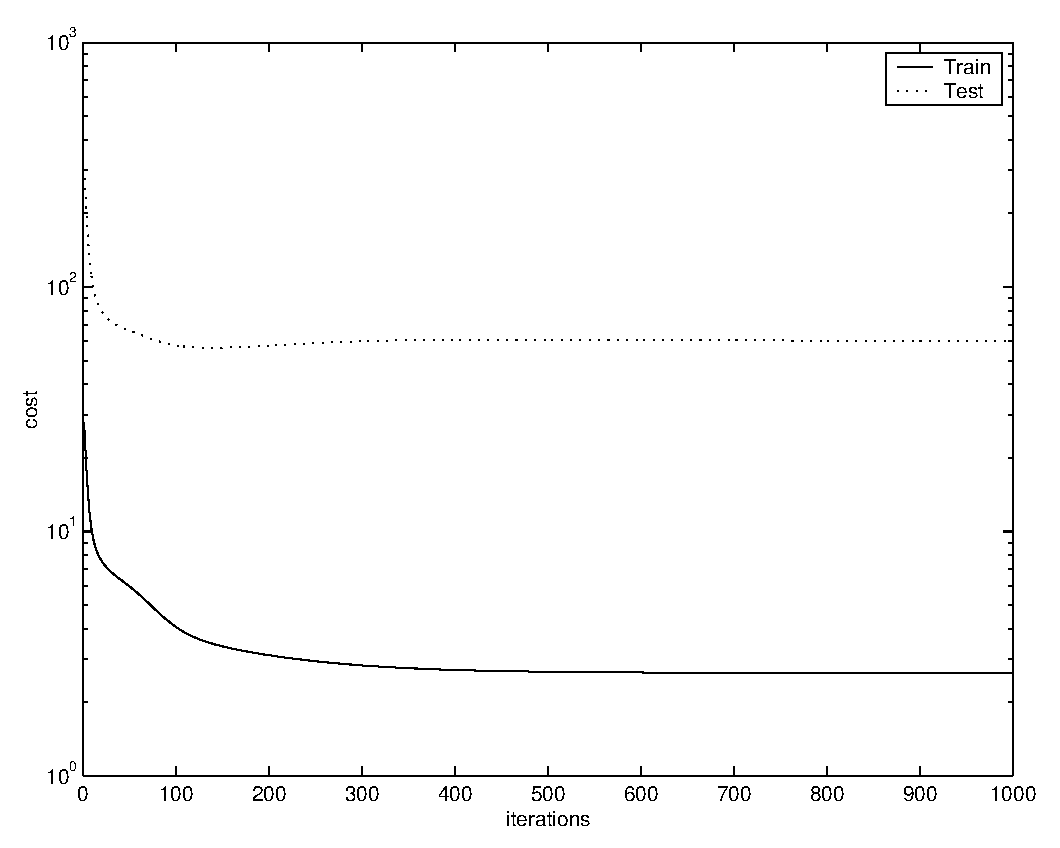
\includegraphics[width=12cm]{cost1.eps}
\caption{Optimization in checkpoint 4.3 showing the train and test
error .} \label{cost1.eps}
\end{figure}

\begin{figure}[ht]
\center
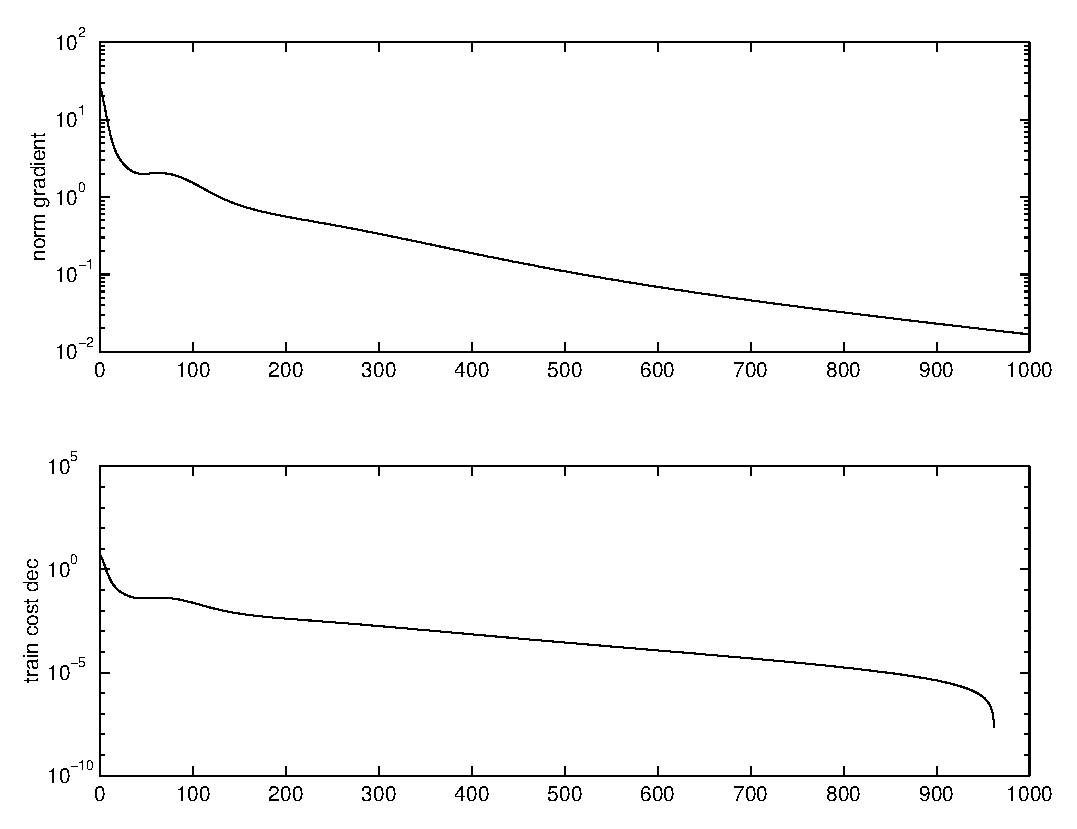
\includegraphics[width=12cm]{cost1grad.eps}
\caption{Optimization in checkpoint 4.3 showing the norm of the
gradient and the difference of the train error between
iterations.} \label{cost1grad.eps}
\end{figure}
